\documentclass{standalone}

\usepackage{tikz}
\usepackage{circuitikz}

\tikzset{block/.style = {draw, fill=white, very thick, rectangle, minimum height=1cm, minimum width=2cm},
         lblock/.style={draw,fill=white,very thick, rectangle, minimum height=3cm, minimum width=1cm},
         sum/.style= {draw, fill=white, very thick, circle, node distance=0.5cm}}

         
\begin{document}
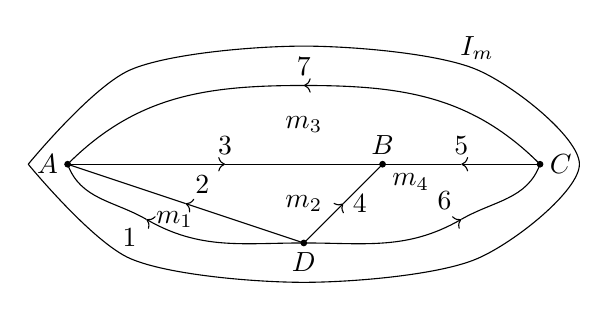
\begin{tikzpicture}
    \filldraw[black](0,0)circle(1pt);
    \filldraw[black](4,0)circle(1pt);
    \filldraw[black](6,0)circle(1pt);
    \filldraw[black](3,-1)circle(1pt);

    \draw[-](0,0)node[left]{$A$}to[out=45,in=180](3,1)node[above]{$7$};
    \draw[<-](3,1)to[out=0,in=135](6,0);
    \node[]at(3,0.5){$m_3$};

    \draw[->](0,0)--(2,0)node[above]{$3$};
    \draw[-](2,0)--(4,0);

    \draw[-](4,0)node[above]{$B$}node[below right]{$m_4$}--(5,0)node[above]{$5$};
    \draw[<-](5,0)--(6,0)node[right]{$C$};

    \draw[->](3,-1)node[below]{$D$}to[out=180,in=330](1,-0.7)node[below left]{$1$}node[right]{$m_1$};
    \draw[-](1,-0.7)to[out=150,in=290](0,0);
    \node[]at(3,-0.5){$m_2$};

    \draw[->](3,-1)--(1.5,-0.5)node[above right]{$2$};
    \draw[-](1.5,-0.5)--(0,0);

    \draw[->](3,-1)--(3.5,-0.5)node[right]{$4$};
    \draw[-](4,0)--(3.5,-0.5);

    \draw[->](3,-1)to[out=0,in=210](5,-0.7)node[above left]{$6$};
    \draw[-](5,-0.7)to[out=30,in=250](6,0);

    \draw[-]plot[smooth]coordinates{(-0.5,0)(0.8,-1.2)(3,-1.5)(5.2,-1.2)(6.5,0)(5.2,1.2)(3,1.5)(0.8,1.2)(-0.5,0)};
    \node[above]at(5.2,1.2){$I_m$};
\end{tikzpicture}
\end{document}